\documentclass[letterpaper, 10 pt, journal, twoside]{IEEEtran} 
% Use this command for final RAL version
%
\usepackage{amsmath}
\usepackage{bm}
\usepackage{breqn}
\usepackage{amssymb}
\usepackage{subcaption}
\usepackage{graphicx}
\usepackage{color}
\usepackage[usenames,dvipsnames,svgnames,table]{xcolor}
\usepackage{tabularx}
\usepackage{multirow}
\usepackage{url}
\usepackage{enumitem}   
\usepackage{xcolor}
\usepackage{makecell}
\usepackage{adjustbox}
\usepackage{booktabs}


\usepackage{hyperref}
\hypersetup{
    colorlinks=true,
    urlcolor=blue,
    citecolor=cyan,}
    

\usepackage{adjustbox}

%\overrideIEEEmargins
% Comment this command for final RAL version.
% Use this command for initial and revised RAL versions, and for final conference version

\newcommand\inputfile[1]{%
  \InputIfFileExists{#1}{}{\typeout{No file #1.}}%
}
\newcommand{\todo}[1]{\noindent\textbf{\textcolor{red}{[TODO: #1]}}}


\makeatletter
\DeclareRobustCommand\icgonedot{\futurelet\@let@token\@icgonedot}
\newcommand\@icgonedot{\ifx\@let@token.\else.\null\fi\xspace}
\newcommand\eg{\textit{e.g., }}
\newcommand\Eg{\textit{E.g., }}
\newcommand\ie{\textit{i.e., }} 
\newcommand\Ie{\textit{I.e., }}
\newcommand\ia{\textit{i.a., }}
\newcommand\Ia{\textit{I.a. ,}}
\newcommand\cf{\textit{cf}} 
\newcommand\Cf{\textit{C.f.}}
\newcommand\etc{\textit{etc.}}
\newcommand\vs{\textit{vs.}}
\newcommand\wrt{w.r.t.}
\newcommand\aka{a.k.a.}
\newcommand\dof{d.o.f.}
\newcommand\etal{et al.}
\newcommand\OFC{\textrm{OFC}\xspace}

%Added by thomas
\newcommand{\mbf}[1]{\mathbf{#1}}
\newcommand{\xb}{\mbf{x}}
\newcommand{\Xb}{\mbf{X}}
\newcommand{\yb}{\mbf{y}}
\newcommand{\zb}{\mbf{z}}
\newcommand{\hb}{\mbf{h}}
\newcommand{\ub}{\mbf{u}}
\newcommand{\Wk}[1]{\mbf{W}_k^{#1}}
\newcommand{\xbp}{\mbf{x^\prime}}
\newcommand{\txb}{\mbf{\tilde{x}}}
\newcommand{\txbp}{\mbf{\tilde{x}^\prime}}
\newcommand{\T}[1]{#1^\mathsf{T}}
\newcommand{\RR}{I\!\!R}
\newcommand{\Mbb}{\mathbb{M}}
\newcommand{\Obb}{\mathbb{O}}
\newcommand{\Zbb}{\mathbb{Z}}
\newcommand{\Ybb}{\mathbb{Y}}
\newcommand{\Rbb}{\mathbb{R}}


\makeatother

%\newcommand\eg{\textit{e.g}\icgonedot}
\begin{document}

\title{Fashion-MNIST Image Classification}


\author{Paolo Leopardi1}


\maketitle

\begin{abstract}
Image Classification è il processo che consente di classificare un'immagine rispetto al contenuto informativo della stessa,assegnandole quindi un qualche significato semantico. Il dataset utilizzato per lo sviluppo del progetto è Fahion-MNIST, questo è costituito da immagini di indumenti di vario tipo. Viene proposto un approccio tramite tecniche di deep learning utilizzando due differenti tipi di reti neurali convoluzionali: il primo modello è stato implementato da zero, il secondo è invece un'architettura di riferimento nel campo delle reti convoluzionali. I risultati mostrano come un modello convoluzionale piuttosto semplice riesca ad ottenere dei risultati molto soddisfacenti evidenziando ancora una volta la potenza delle reti neurali. 
\end{abstract}

\IEEEpeerreviewmaketitle
\section{Introduction} \label{sec:introduction}
Il task di Image Classification consiste nell'assegnare ad un'immagine una specifica etichetta scelta fra un set di label disponibili. Le immagini di cui si compone il dataset dovranno raffigurare perciò un solo elemento fra quelli associabili ad una delle classi. A differenza di altri task tipici della Computer Vision questo non richiede alcuna localizzazione degli elementi presenti nell'immagine; basti pensare ad esempio all'Object Detection and Recognition in cui, oltre alla classificazione dell'oggetto presente nell'immagine, si devono fornire anche le coordinate della boundig box che lo racchiude.\par
In questo progetto è stato impiegato il dataset Fashion-MNIST \cite{xiao2017fashion}, liberamente scaricabile da
\href{https://github.com/zalandoresearch/fashion-mnist}{GitHub}. Quest'ultimo è costituito da immagini grayscale 28x28 di capi d'abbigliamento provenienti dal sito di e-commerce \href{https://www.zalando.it/}{Zalando} (Figura \ref{fig1:fashion-MNIST}) classificati in classi da 0 a 9 nel seguente ordine: T-shirt/top, Trouser, Pullover, Dress, Coat, Sandal, Shirt, Sneaker, Bag, Ankle boot.
\begin{figure}[!hbt]
    \centering
    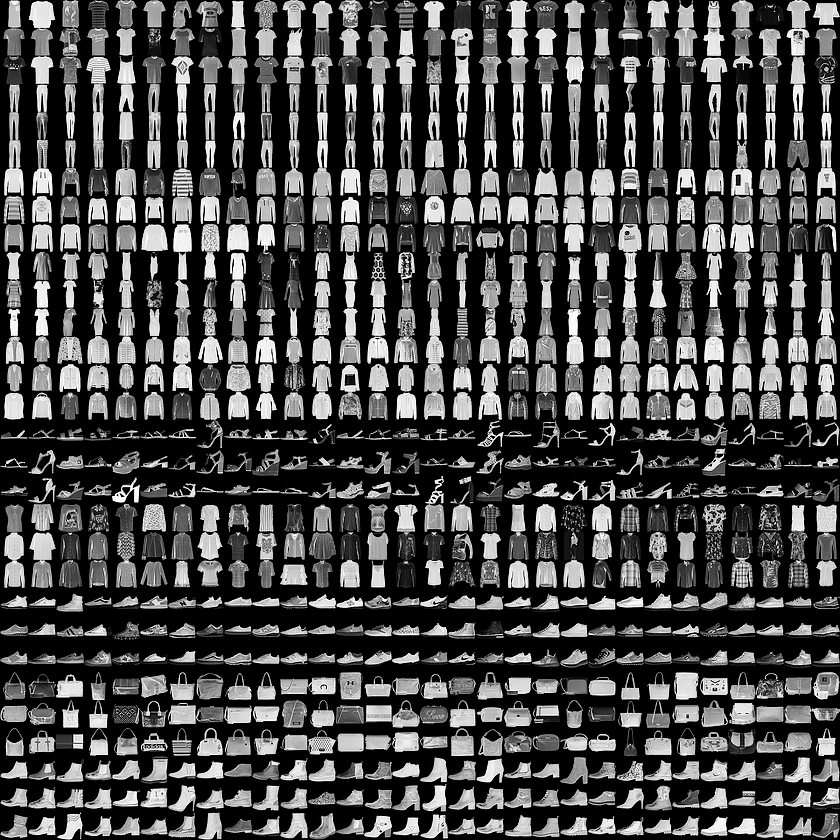
\includegraphics[width=\columnwidth]{images/fashion-mnist-sprite.png}
    \caption{Immagini estratte dal dataset Fashion-MNIST (tre righe per classe)}
    \label{fig1:fashion-MNIST}
\end{figure}
La nascita di Fashion-MNIST è dovuta al sovrautilizzo del noto dataset MNIST database of handwritten digit  \cite{lecun1998mnist}, utilizzato come punto di riferimento dalla comunità scientifica. Gli autori infatti spiegano che MNIST handrwitten è un dataset "troppo facile" dato che le reti convoluzionali riescono a raggiungere un punteggio del 99,7\% ed anche gli algoritmi classici di Machine Learning riesco a ottenere facilmente score del 97\%. L'esperto di deep learning François Chollet, creatore di Keras \cite{chollet2015keras}, ha dichiarato nell'Aprile del 2017 attraverso il proprio profilo \href{https://twitter.com/fchollet/status/852594987527045120}{Twitter} che MNIST non è rappresentativo dei moderni task di CV.\par
Per il task in questione sono state utilizzate due soluzioni architetturali differenti di reti neurali convoluzionali, le reti di questo tipo sono infatti disegnate per processare i dati disposti a griglia (come accade per i pixel di un'immagine). Una rete convoluzionale è un caso speciale di rete neurale che utilizza la convoluzione in almeno uno dei suoi layer. Le architetture proposte sono:
\begin{itemize}
\item CustomNet
\item ResNet-18 \cite{he2016deep}
\end{itemize}
CustomNet è un'architettura molto semplice progettata da zero ed è costituita da 3 layer convoluzionali e da un ultimo layer fully connected. ResNet-18 è invece il modello proposto da He \etal{} opportunamente riadattato per lo specifico compito in questione.\par
Infine sono state testate le soluzioni architetturali proposte valutandone le performance grazie alle metriche di accuracy, precision e recall.

\section{Related Work} \label{sec:related_work}
Ad oggi esistono varie architetture convoluzionali fondamentali che sono divenute famose nel corso degli anni, ognuna avente le sue peculiarità; molte di queste sono state utilizzate per task di Image Classification: LeNet-5 \cite{lecun1998gradient}, AlexNet \cite{krizhevsky2012imagenet}, VGGNet\cite{simonyan2014very}. Le reti sopracitate insieme ad altre sono state valutate anche in Fashion-MNIST da Y.Zhang in un articolo pubblicato nel 2019 \cite{zhang2019evaluation}.\par
Oltre alle architetture fondamentali vengono proposti innumerevoli pattern che riescono ad ottenere degli ottimi risultati. Ad esempio il modello sviluppato da Duan \etal{} \cite{duan2019image} basato su VGG ha raggiunto un'accuracy del 91,5\%. Un'altra soluzione realizzata da Bhatnagar \etal{} \cite{bhatnagar2017classification} ha ottenuto il 92,54\%.
\section{Proposed Approach} \label{sec:approach}
Il dataset prevede 60.000 campioni di training e 10.000 di test, è stato però necessario ridurre il numero di sample per il training set così da avere delle tempistiche ragionevoli per effettuare l'addestramento delle reti. Sono quindi stati estratti i primi 5.000 sample per il training e di conseguenza la dimensione del test set è stata portata a 1.000 campioni. Come mostrato nelle Figure \ref{fig2:train_sample_distribution} e \ref{fig3:test_sample_distribution} la distribuzione delle etichette rimane comunque bilanciata sia nel training che nel test set.
\begin{figure}[!hbt]
    \centering
    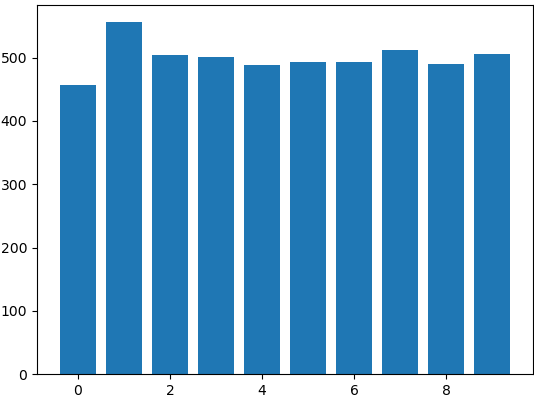
\includegraphics[width=\columnwidth]{images/train_sample_distribution2.png}
    \caption{Distribuzione label training set dopo la riduzione del dataset}
    \label{fig2:train_sample_distribution}
\end{figure}

\begin{figure}[!hbt]
    \centering
    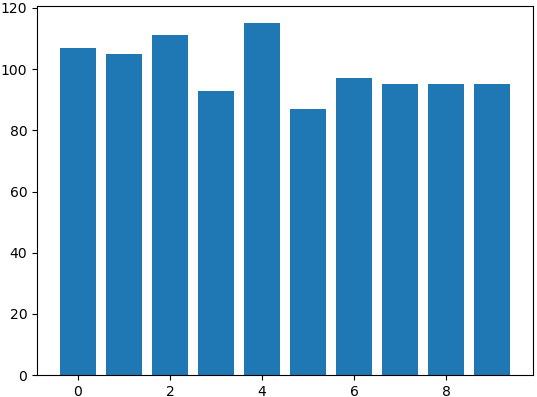
\includegraphics[width=\columnwidth]{images/test_sample_distribution2.png}
    \caption{Distribuzione label test set dopo la riduzione del dataset}
    \label{fig3:test_sample_distribution}
\end{figure}


\subsection*{CustomNet}
L'architettura (Figura \ref{fig4:custom_net_architecture}) è costituita da tre blocchi convoluzionali, i primi due del tutto identici fra loro, il terzo è stato leggermente modificato rispetto  ai precedenti:
\begin{enumerate}
\item \textbf{Convolutiona layer}\\
\-\ input ch: 1\\ \-\ out ch: 32\\ \-\ kernel_size: $3\times3$\\ \-\ stride: 1\\ \-\ padding: 1
\item \textbf{Batch Normalization}
\item \textbf{ReLU}
\item \textbf{Max Pooling 2D}\\
\-\ kernel size: $2\times2$\\ \-\ stride: 2

\item \textbf{Convolutional layer}\\
\-\ input ch: 32\\ \-\ out ch: 64\\ \-\ kernel_size: $3\times3$\\ \-\ stride: 1\\ \-\ padding: 1
\item \textbf{Batch Normalization}
\item \textbf{ReLU}
\item \textbf{Max Pooling 2D}\\
\-\ kernel size: $2\times2$\\ \-\ stride: 2

\item \textbf{Convolutional layer}\\
\-\ input ch: 64\\ \-\ out ch: 128\\ \-\ kernel_size: $3\times3$\\ \-\ stride: 1\\ \-\ padding: 1
\item \textbf{Batch Normalization}
\item \textbf{ReLU}
\item \textbf{Dropout}\\
\-\ probability: 0.5
\item \textbf{Fully connected}\\
\-\ in size: 6272\\ \-\ out size: 10
\end{enumerate}
\begin{figure}[!hbt]
    \centering
    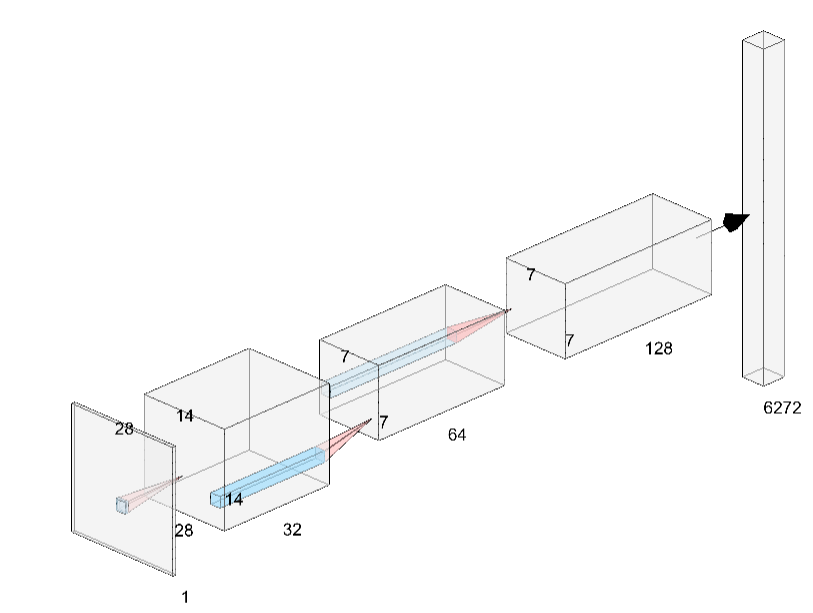
\includegraphics[width=\columnwidth]{images/CustomNetArchitecture.png}
    \caption{Architettura CustomNet}
    \label{fig4:custom_net_architecture}
\end{figure}
In tutti i blocchi la dimensione del kernel è $3\times3$, impilare layer convoluzionali con kernel di dimensioni ridotte consente di avere una maggior espressività delle feature ed un minor numero di parametri rispetto ad un unico layer convoluzionale avente un kernel di dimensioni maggiori. \`{E} stato sempre applicato il padding same  così da non ridurre la dimensione del tensore in input al blocco successivo a seguito della convoluzione. Successivamente è stato inserito il layer di batch normalization così da normalizzare l'output della convoluzione che poi andrà in input alla funzione di attivazione. ReLU (Rectified Linear Unit) è una funzione non lineare definita come:
$$f(x) = max(0,x)$$
Nei primi due blocchi è stato applicato un max pooling, questo consente di ottenere una statistica sommaria degli output del layer precedente nell'intorno del pixel e una rappresentazione invariante a piccole traslazioni dell'input. I parametri impostati per il pooling dimezzano la dimensione del volume in ingresso. In Figura \ref{fig4:custom_net_architecture} è mostrato un esempio di applicazione di max pooling.
\begin{figure}[!hbt]
    \centering
    \includegraphics[width=\columnwidth]{images/MaxPoolSample2.png}
    \caption{Applicazione max pooling con kernel $2\times2$ e stride 2}
    \label{fig5:max_pooling}
\end{figure}
Nell'ultimo blocco al posto del max pooling è stato introdotto  un layer di dropout \cite{srivastava2014dropout} per effettuare la regolarizzazione e quindi prevenire l'overfitting.Il dropout è una tecnica di regolarizzazione estremamente efficace che consiste nel mantenere un neurone attivo con probabilità $p$, questo si traduce in fase di training con l'eliminazione di alcune connessioni randomicamente in base a $p$. Così facendo la rete utilizza un numero di parametri inferiore e non sapendo a priori quali connessioni verranno inibite è costretta ad apprendere i concetti veramente importanti. Infine vi è il layer fully connected che produce in uscita la predizione, chiaramente è stato necessario effettuare precedentemente la vettorializzazione del tensore.
\subsection*{Resnet-18}
Essendo Resnet-18 un'architettura fondamentale non è stato necessario implementarla da zero, tuttavia la struttura è stata modificata in alcuni punti per adattarla al task in questione. \`{E} stato sostituito il primo layer convoluzionale dato che questo prende in input immagini RGB, quindi aventi 3 canali. Il nuovo layer, sempre convoluzionale, ha gli stessi parametri dell'originale fatta eccezione per la dimensione dell'input che passa da 3 a 1. A valle della rete l'ultimo layer fully connected è stato modificato per avere l'uscita di dimensione pari al numero delle classi, cioè 10.\par
\`{E} stata scelta questa rete essendo uno standard attuale che  rappresenta la backbone delle moderne reti neurali, è stato inoltre il progetto vincitore nel 2015 di ILSVRC \cite{ILSVRC15} (ImageNet Large Scale Visual Recognition Challenge).
\begin{figure}[!hbt]
    \centering
    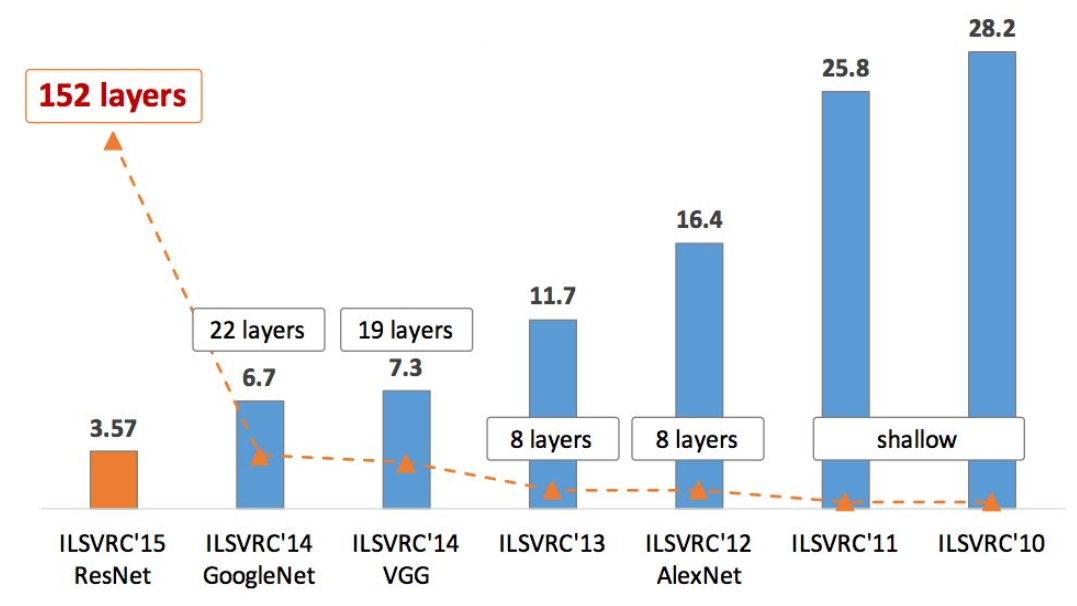
\includegraphics[width=\columnwidth]{images/ilsvrc_winners.png}
    \caption{Vincitori di ILSVRC dal 2010 al 2015}
    \label{fig6:ILSVRC2015}
\end{figure}\par
L'elemento caratterizzante di questa rete sono i residual block: questi consento al gradiente di propagarsi all'indietro nella rete senza essere alterato cosi da scongiurare il problema del \textit{vanishing gradient}.




  
\section{Experiments} \label{sec:experiments}
\subsection*{Training}
Entrambe le reti sono state addestrate per 30 epoche utilizzando la cross-entropy loss. CustomNet è stata addestrata da zero e la Figura \ref{fig7:layer1_filter} mostra i filtri del primo layer convoluzionale al termine dell'addestramento. 
\begin{figure}[!hbt]
    \centering
    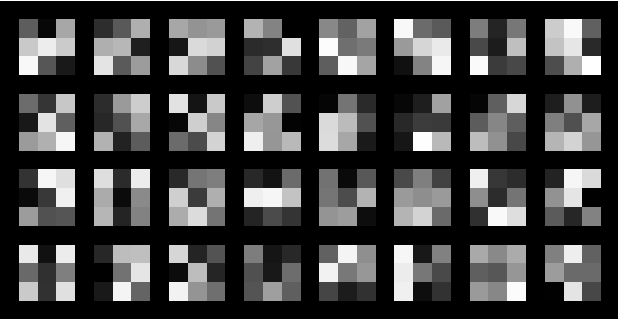
\includegraphics[width=\columnwidth]{images/layer1_filter.png}
    \caption{Filtri del primo layer convoluzionale di CustomNet ottenuti al termine della fase di training}
    \label{fig7:layer1_filter}
\end{figure}\par
La figura \ref{fig8:feature_map} mostra la decima feature map per ogni layer convoluzionale; la prima immagine mostra l'input, in questo caso corrispondente alla classe Coat (4). Si osserva come man mano che si scende in profondità la rete impara ad estrarre l'oggetto presente e distinguerlo dal background.
\begin{figure}[!hbt]
    \centering
    \includegraphics[width=\columnwidth]{images/customNet_featureMap2.png}
    \caption{Input e feature map dei layer convoluzionali}
    \label{fig8:feature_map}
\end{figure}\par
Per quanto riguarda Resnet sono stati addestrati solo i layer alterati rispetto alla struttura originale, essendo la rete preaddestrata con il dataset ImageNet \cite{deng2009imagenet}. Grazie a questa procedura di transfer learning è stato possibile utilizzare la rete che altrimenti avrebbe richiesto un tempo eccessivo per la fase di training.
\subsection*{Risultati}
Per valutare le performance delle reti è stata utilizzata l'accuracy, questa consente di individuare la percentuale di classificazioni corrette sul totale delle predizioni. \`{E} definita come:$$Accuracy = \frac{predizioni\: corrette}{predizioni\: totali}$$ Le Figure \ref{fig9:customNet_score} e \ref{fig10:resNet_score} mostrano l'andamento dell'accuracy su train e test set per entrambi i modelli all'avanzare delle epoche. CustomNet riesce a raggiungere un'accuracy del 91\% sul train set e dell'88\% sul test. Resnet-18 ottiene dei risultati inferiori arrivando ad un 74\% sul training e un 68\% sul test.
\begin{figure}[!hbt]
    \centering
    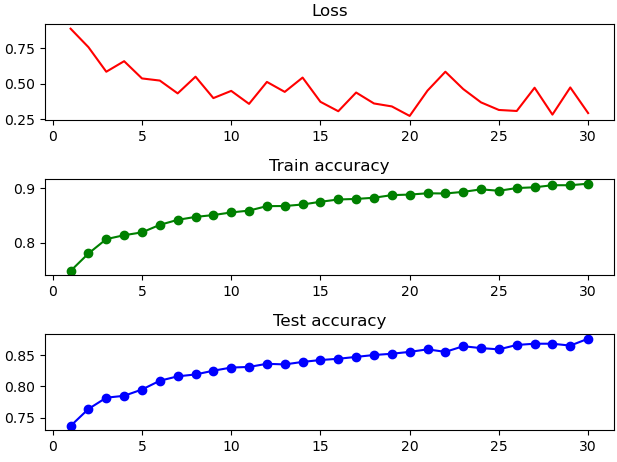
\includegraphics[width=\columnwidth]{images/CustomNetScore1bis.png}
    \caption{Andamento di loss, train accuracy e test accuracy utilizzando CustomNet}
    \label{fig9:customNet_score}
\end{figure}
\begin{figure}[!hbt]
    \centering
    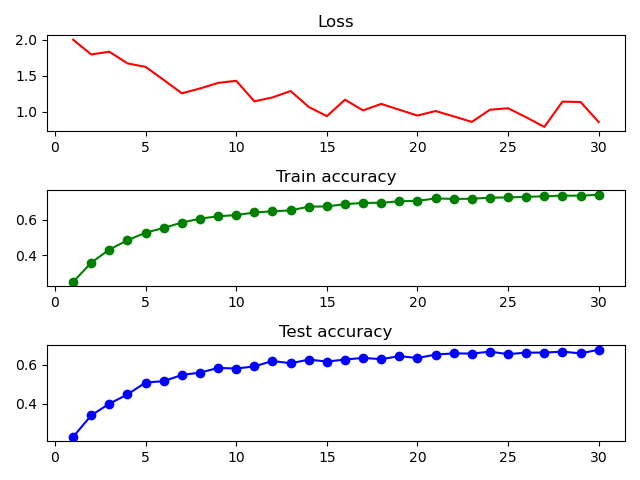
\includegraphics[width=\columnwidth]{images/ResNetScore.png}
    \caption{Andamento di loss, train accuracy e test accuracy utilizzando ResNet-18}
    \label{fig10:resNet_score}
\end{figure}\par
Sono state inoltre calcolate precision e recall per le singole classi:
$$Precision = \frac{TP}{TP+FP} \quad Recall=\frac{TP}{TP+FN}$$
La precision indica la proporzione di predizioni positive corrette rispetto a tutte le predizioni positive. La recall indica invece la proporzione di predizioni positive corrette rispetto a tutti i campioni effettivamente positivi. In un task di classificazione multiclasse si assegna la classe positiva ad una sola etichetta e al resto delle label viene assegnata la classe negativa.
\begin{table}[!hbt]
\centering
\begin{adjustbox}{width=\columnwidth}
\begin{tabular}{|l|c|c|c|c|}
\hline        & \multicolumn{2}{c|}{\textbf{CustomNet}}& \multicolumn{2}{c|}{\textbf{ResNet-18}}\\
\hline \textbf{Label} &\textbf{Precision} &\textbf{Recall} &\textbf{Precision} &\textbf{Recall} \\
\hline 0: T-shirt/Top & 0.85& 0.90 & 0.67&0.73\\
\hline 1: Trouser     & 0.98& 0.99 & 0.90&0.81\\
\hline 2: Pullover    & 0.82& 0.81 & 0.54&0.43\\
\hline 3: Dress       & 0.84& 0.85 & 0.67&0.64\\
\hline 4: Coat        & 0.83& 0.86 & 0.52&0.65\\
\hline 5: Sandal      & 0.89& 0.94 & 0.76&0.80\\
\hline 6: Shirt       & 0.76& 0.68 & 0.34&0.37\\
\hline 7: Sneaker     & 0.92& 0.90 & 0.85&0.84\\
\hline 8: Bag         & 0.95& 0.96 & 0.75&0.79\\
\hline 9: Ankle boot  & 0.95& 0.92 & 0.82&0.82\\
\hline
\end{tabular}
\end{adjustbox}
\label{tab1:precision-recall}
\caption{Precision e recall calcolate sul test set}
\end{table}\par
Infine è stata visualizzata la confusion matrix per CustomNet riguardante le predizioni effettuate sul test set. Grazie a questa si riesce a capire quali classi siano più difficili da disambiguare per la rete. La diagonale principale rappresenta il numero di predizioni corrette per ogni classe, mentre invece i valori fuori diagonale rappresentano una predizione sbagliata.
\begin{figure}[!hbt]
    \centering
    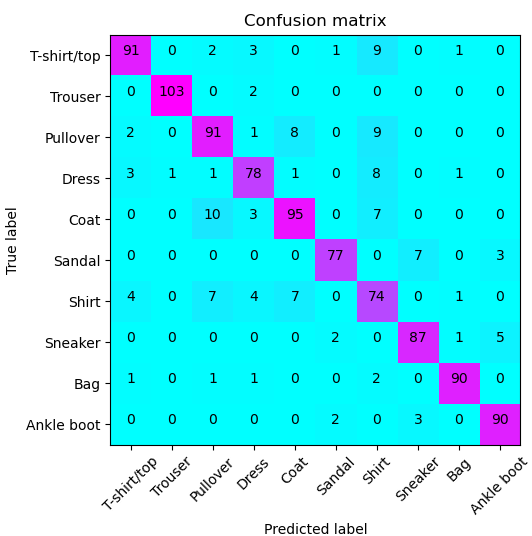
\includegraphics[width=\columnwidth]{images/confusion_matrix1.png}
    \caption{Confusion matrix per le predizioni di CustomNet sul test set}
    \label{fig11:confusion_matrix}
\end{figure}


\section{Conclusion} \label{sec:conclusions}
I risultati ottenuti evidenziano come CustomNet seppur essendo una rete piuttosto semplice riesca comunque a realizzare dei buoni score. Riguardo ResNet invece i risultati sono significativamente inferiori, tuttavia bisogna tener sempre in considerazione che la rete è stata scaricata preaddestrata su immagini di tipo RGB provenienti da un altro dataset; solamente il primo e l'ultimo layer sono stati addestrati sul training set di Fahion-MNIST.\par
Entrambe le reti mostrano comunque una forte insofferenza rispetto alla classe numero 6, ovvero Shirt. Come si può vedere dalla confusion matrix questa viene confusa da CustomNet con le classi T-shirt/top, Pullover, Dress e Coat. La figura \ref{fig12:abiti_example} mostra un esempio di queste classi e si intuisce come ad esempio le classi Shirt e T-shirt/top possano risultare molto simili.
\begin{figure}[!hbt]
\centering
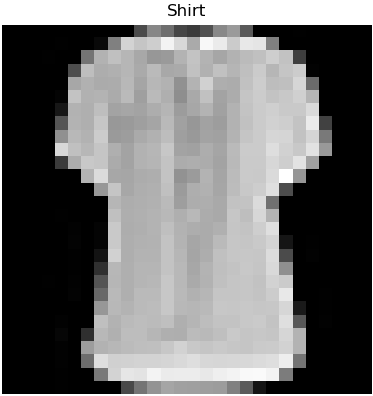
\includegraphics[width=4cm]{images/shirt6bis.png}
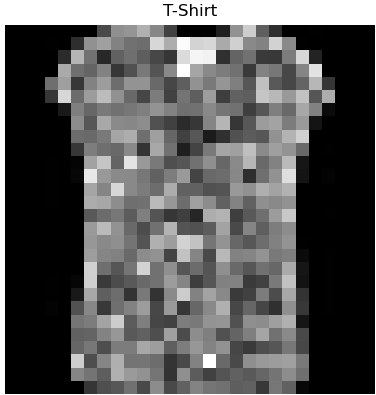
\includegraphics[width=4cm]{images/tshirt0bis.png}
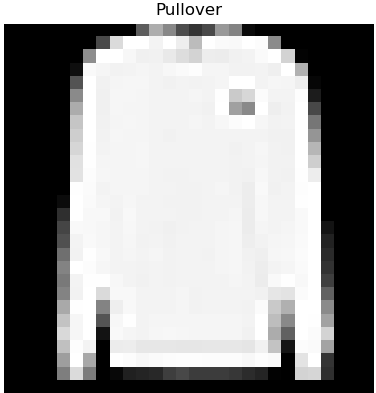
\includegraphics[width=4cm]{images/pullover2bis.png}
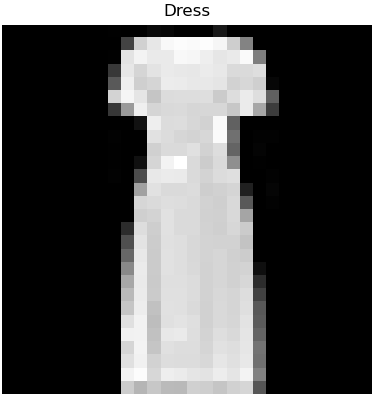
\includegraphics[width=4cm]{images/dress3bis.png}
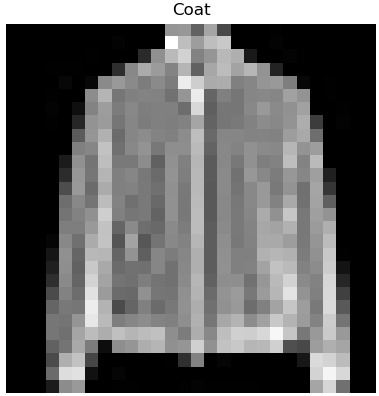
\includegraphics[width=4cm]{images/coat4bis.png}
\caption{Esempi di immagini per le classi Shirt, T-shirt/top, Pullover, Dress e Coat}
\label{fig12:abiti_example}
\end{figure}
La rete riesce invece a distinguere bene le classi riguardanti le calzature (Sandal, Sneaker, Ankle boot) seppur possano sembrare analoghe fra loro in alcuni casi.
\begin{figure}[!hbt]
\centering
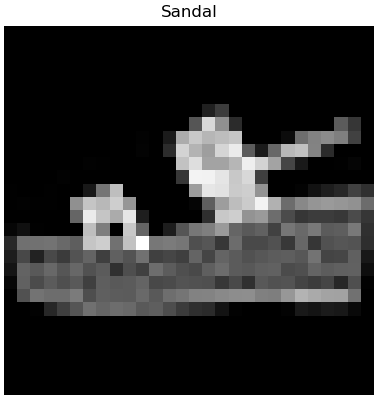
\includegraphics[width=4cm]{images/sandal5bis.png}
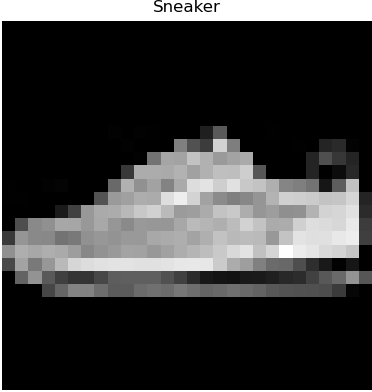
\includegraphics[width=4cm]{images/sneaker7bis.png}
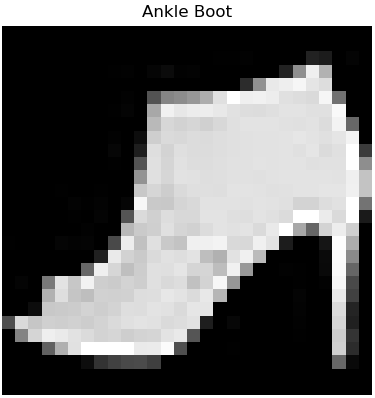
\includegraphics[width=4cm]{images/ankleboot9bis.png}
\caption{Esempi di immagini per le classi Sandal, Sneaker, Ankle boot}
\label{fig13:scarpe_example}
\end{figure}
Le immagini raffiguranti le label Trouser e Bag vengono classificate sempre in maniera corretta fondamentalmente. I due indumenti hanno infatti delle forme molto differenti rispetto alle altre classi, basta infatti osservare la Figura \ref{fig1:fashion-MNIST} a monte del documento per comprenderne le differenze.




%\begin{acknowledgements}
%If you'd like to thank anyone, place your comments here
%and remove the percent signs.
%\end{acknowledgements}

% BibTeX users please use one of
%\bibliographystyle{spbasic}      % basic style, author-year citations
%\bibliographystyle{spmpsci}      % mathematics and physical sciences
\bibliographystyle{IEEEtran}       % APS-like style for physics
\bibliography{bibliography}   % name your BibTeX data base


\end{document}
% end of file template.tex

